\chapter{Introduction}

%Reachi is a coordinated effort to enable vital communication during emergencies such as natural disasters, where earthquakes, tsunamis, forest fires, and more, destroy the pre-existing communication infrastructure, rendering it near impossible to organise the relief effort to effectively aid the affected, assess the damage, as well as organising repairs to the damaged infrastructure. The goal of the Reachi project is to optimise the disaster response by creating an overview of the situation within the first eight hours after the disaster. Today, this process can take up 1-2 weeks, due to the destruction of pre-existing communication infrastructure~\cite{website:reachiproject}. Without this overview, it is impossible to know where the needs for disaster relief is greatest, or what the level of disaster relief is even available. The project has been developed by the danish company LinkAiders ApS, and utilise a technology to enable mobile ad-hoc mesh networking through radio communication, created by NeoCortec.

%\begin{figure}[H]
%    \centering
%    \begin{subfigure}[]{.2\textwidth}
%        \qrcode[hyperlink,height=1.0in]{https://www.youtube.com/watch?v=Hh2Cw6GhBRU}
%        %\caption{2000 nodes.}
%        \label{figure:clustering:2knodes}
%    \end{subfigure}
%    \begin{subfigure}[]{.79\textwidth}
%        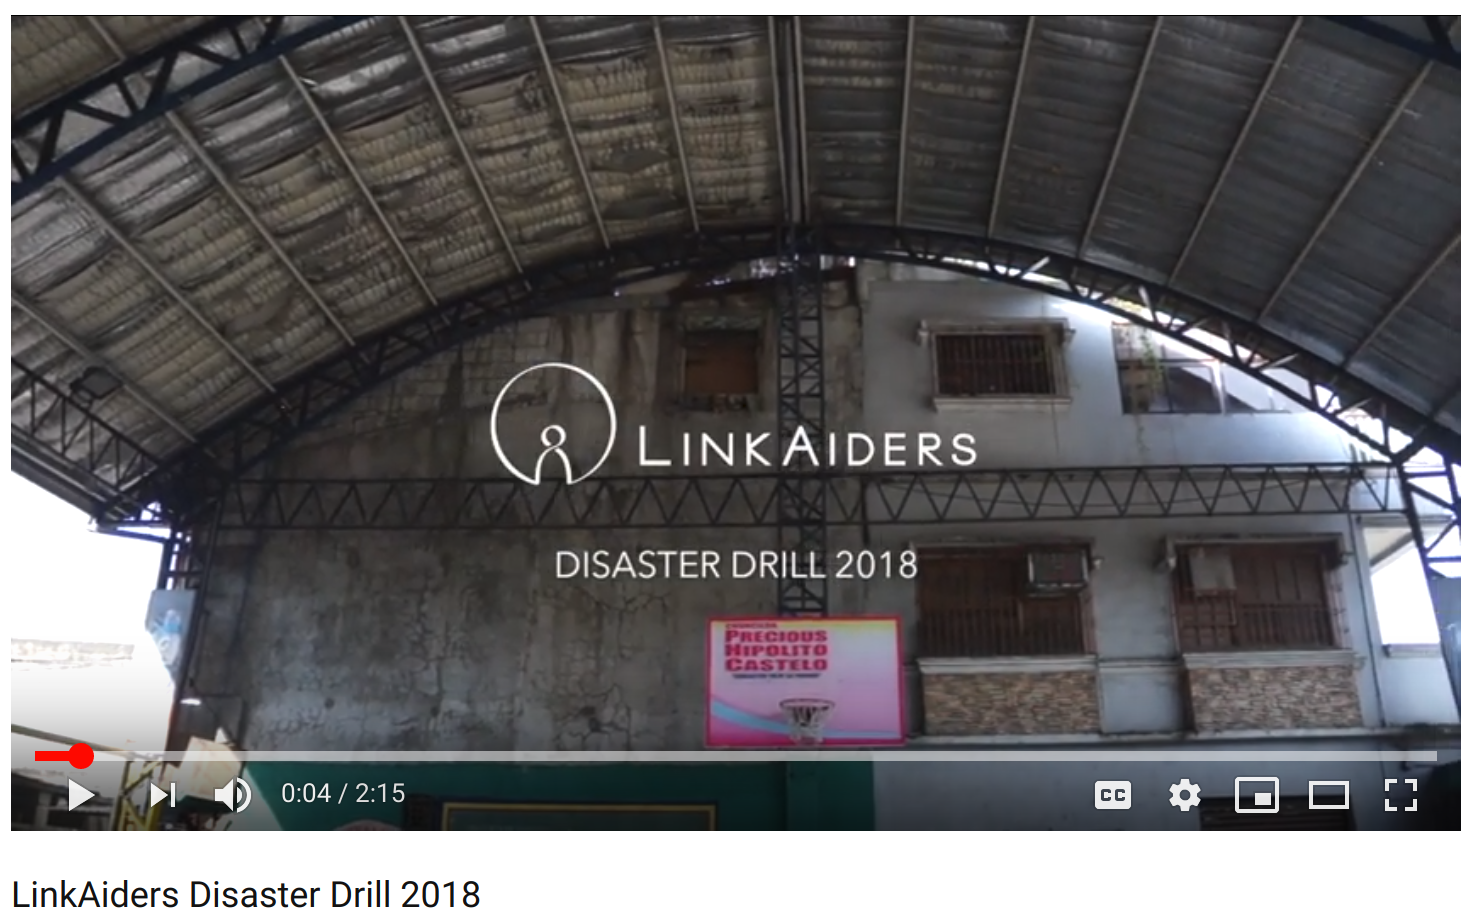
\includegraphics[width=\linewidth]{figures/linkaiders-drill-320.png}
%        %\caption{2000 nodes clustered.}
%        \label{figure:clustering:2k80m2ptsnodes}
%    \end{subfigure}
%    \caption{A YouTube video, showing the largest scale drill of the Reachi project with 320 volunteers.}
%    \label{figure:introduction:reachi-test}
%\end{figure}

%To date, the largest scale drill of the Reachi system was conducted in September 2018, in the Phillippines, with the help of 320 volunteers. The drill was conducted in order to test the Reachi system as a needs assessment tool, the volunteers' ability to use the Reachi devices, as well as the ability of the Reachi system to create the necessary overview of the situation, in less than eight hours. A video of the drill has been uploaded to the LinkAiders ApS YouTube channel, and the link is encoded in the QR Code in \autoref{figure:introduction:reachi-test}. \medbreak

%The goal for the Reachi project is to scale, and test, the project with up to 1000 devices~\cite{website:reachiproject}, which is a massive undertaking, and would require even more effort to organise such a drill. 
% https://www.youtube.com/watch?v=Hh2Cw6GhBRU

% https://markedsmodningsfonden.dk/reachi-vital-informationsdeling-i-katastrofesituationer

The goal of the project is to simulate wireless network protocols for communication in a mobile setting. Testing the capabilities of a wireless network protocol can prove to be a challenge when testing with physical units in a real-life scenario.

Simulation as an alternative to testing with physical units: Scalability, repeatability, simulating different scenarios.

%%%%%%%%%%%%%%%%%%%%%%%%%%%%%%%%%%%%%%%%%%%%%%%%%%%%%%%%%%%%%%%%%%%%%%%%%%%%%%%%%%%%%%%%%%
% Basically description env uden env
When testing \gls{manet} protocols, or just network protocols in general, scale is important. 

Testing the protocol on a network of the size of a real world scenario gives the best insight in the behaviour of the protocol.

Even better would be to test on a network larger than anticipated, to stress test and observe worst case scenarios.

Another problem accompanied with the scaling problem, is the physical devices that are to be used for the test. 

Testing with the devices that the protocol will be deployed with, is the ideal scenario, but that is not always possible. 

Fabricating the devices is both expensive and time consuming, e.g. the desired network size is 1000 nodes. Then 1000 devices would have to be fabricated and set up.

Another problem is repeatability. To run a test with physical devices, test personal is needed. 

The test personal will have to move around in the world, in predefined patterns to test several different network topologies. 
When a lot of people is involved it gets complicated to keep everything coordinated, whilst no guarantee that when the test is repeated, the test personal will behave in the exact same way thereby not producing consistent test results.\medbreak

To solve the above mentioned issues, this paper intends to develop a framework for simulating \gls{manet} protocols. 

The framework will emulate the physical devices that would normally run the \gls{manet} protocol, on Aalborg University's compute cluster. 

Each emulated unit, is emulated as a process in a \gls{mpi} setting, allowing one to emulate a large amount of network nodes. 

Though the size of the cluster decides the possible amount of emulated nodes. 
The hardware will then be simulated, on the emulated devices. 
Since the hardware is entirely software, it allows for simulating any kind of hardware that would be used in physical devices running \gls{manet} protocols.\medbreak


When emulating physical devices, it is important to consider the conditions that the unit are to be used in. 
In the case of devices running \gls{manet} protocols, its that the communication between nodes in the network will influenced by the terrain. 
Bit errors might happen, when transmitting a message over the network, because of obstacles interfering with the signal, hence the framework must also emulate that behaviour.
This is done by calculating the \gls{pep} based on a calculated link model, that will continuously be updated throughout the simulations lifetime.





%  Don't write so much about Reachi. This project was not about Reachi.
%  Motivation should be more general, instead of mentioning neocortec. Mention what the goal of the project is.
%
%  It takes a long time, its complicated to run it in terrain. Testing on real devices is expensive, repeatability is a problem.
%  Scalability is a big challenge, repeatability is another. The possibility to simulate different scenarios, where it would be difficult to instruct volunteers to perform these scenarios.
%
%  We emulate the physical devices, where the hardware is simulated by software.
%
%  Be very clear of what we are actually doing!
%  What is simulated, what is emulated, and how do we deal with these issues?
%
%  Try to avoid things like we will present, or we would like to be able to.
%

Our project proposes a C++ library for writing, and running, simulations of the network protocol behind the mesh communication in a \gls{manet}, using state-of-the-art modelling of link \gls{pathloss} behind the radio communication, to simulate packet loss and collisions caused by interference. With our library, it would be possible to write a C++ implementation of communication protocols, such as \gls{lmac}~\cite{paper:lmac_protocol} or Slotted ALOHA~\cite{Roberts:1975:APS:1024916.1024920}, using a simple interface header file resembling a traditional hardware interface.
